\chapter{(B) Risultati numerici relativi al \textit{pricing} Monte Carlo}
Menzionare i dati <<standard>> delle simulazioni.

\section{(B-1) Controlli di affidabilità dei risultati}
\subsection{(B-1-i) Corrispondenza tra risultati in CPU e GPU} \label{sec:cpugpu}

Per poter verificare che l'algoritmo implementato riproducesse esattamente gli stessi risultati su GPU e CPU è stato adottato il paradigma \textit{host-device}, tecnica che permette di eseguire lo stesso codice su entrambe le architetture senza doverlo duplicare.

A questo scopo è stata definita una funzione generica \codeword{OptionPricingEvaluator_HostDev(...)} nella variante \codeword{__host__ __device__} , eseguibile su entrambi i supporti, che contiene l'algoritmo per il \textit{pricing} delle opzioni. Questa funzione non fa uso di parti specifiche di CUDA e, oltre a dei parametri, riceve in input un indice che identifica il \textit{thread}. Segue la definizione di due ulteriori funzioni \codeword{OptionPricingEvaluator_Host(...)} e  \codeword{OptionPricingEvaluator_Global(...)} con la stessa segnatura di \codeword{OptionPricingEvaluator_HostDev(...)}, ma omettendo il parametro riguardante l'indice. La prima, essendo di tipo \codeword{__host__}, è eseguibile solo su CPU e richiama al suo interno \codeword{OptionPricingEvaluator_HostDev(...)} identificando il valore dell'indice dal ciclo \codeword{for} in cui essa si trova. La seconda, essendo di tipo \codeword{__global__}, è eseguibile solo su GPU e richiama al suo interno \codeword{OptionPricingEvaluator_HostDev(...)} identificando l'indice attraverso la coordinata \codeword{threadIdx.x + blockDim.x * blockIdx.x}. 

Il metodo Monte Carlo si adatta perfettamente a questo paradigma poiché i singoli \textit{thread} eseguono le stesse istruzioni su flussi di dati differenti; l'implementazione su CPU non sarebbe possibile se i singoli \textit{thread} interagissero tra loro. 

\subsection{(B-1-ii) Corrispondenza tra risultati e valori calcolati analiticamente}

Un ulteriore controllo sulla bontà dei risultati ottenuti dalle simulazione consiste nell'effettuare un confronto tra i prezzi Monte Carlo ottenuti per le opzioni \textit{plain vanilla} e per il contratto \textit{forward} e i loro rispettivi valori analitici ottenuti applicando la teoria di Black \& Scholes. 

L'argomentazione di Black \& Scholes permette una derivazione quantitativa di una formula analitica esatta per valutare il prezzo di un'opzione europea \textit{plain vanilla} basandosi su alcune assunzioni. Di conseguenza quest'ultima fornisce uno strumento fondamentale per verificare la correttezza delle simulazioni.

Patendo dai presupposti di Black \& Scholes si ricava l'omonima equazione differenziale alle derivate parziali:
\begin{equation}
    \frac{\partial F}{\partial t} + rS \frac{\partial F}{\partial S} + \frac{1}{2} \sigma ^2 S ^2 \frac{\partial ^2 F}{\partial S^2} = r F
    \label{eq:BS}
\end{equation}
dalla quale è possibile ottenere la formula analitica per il pricing delle opzioni. Nella \ref{eq:BS} $S(t)$ indica il prezzo di un'azione, $F(t)$ il valore di un qualsiasi derivato su cui è costruito l'opzione e con $r$ e $\sigma$ si indicano rispettivamente il tasso di interesse privo di rischio e la volatilità. Si osservi che questa equazione è valida per un generico derivato; la differenza tra un'opzione e un'altra consiste nelle condizioni al contorno che si impongono su $F(t)$ al fine di risolvere l'equazione. In particolare quello caratterizza un'opzione è il medo in cui viene assegnato il \textit{pay-off} sulla base del prezzo raggiunto dal sottostante. Pertanto la condizione al contorno applicata è data da:
\begin{equation}
    F(S,t=T) = Pay-off(S)
    \label{eq:boundarycondition}
\end{equation}
dove $T$ indica la data di maturità.
Il sistema cosi formato dalla \ref{eq:BS} e dalla \ref{eq:boundarycondition} permette di ottenere un'unica soluzione.

Di conseguenza per le opzioni \textit{plain vanilla} si ricava:

\begin{equation}
    F_{call option} = S N(d_{1}) - E \exp{- r T} N(d_{2});
\end{equation}
\begin{equation}
    F_{put option} = S N(d_{1}-1) - E \exp{- r T} N(d_{2}-1)
\end{equation}
dove $S$ è il prezzo del sottostante, $r$ il termine di drift, $E$ il prezzo di esercizio, mentre $N(x)$ indica la funzione di distribuzione normale cumulata:
\begin{equation}
    N(x)= \frac{1}{2}
    (1+erf(\frac{x}{\sqrt{2}})
\end{equation}
valutata in:
\begin{equation}
    d_{1}=\frac{\log(\frac{S}{E}) + (r+\frac{\sigma ^2}{2}) T}{\sigma \sqrt{T}};
\end{equation}
\begin{equation}
    d_{2}=d_{1}- \sigma \sqrt{T}
\end{equation}

Per quanto riguarda il contratto \textit{forward} il risultato analitico coincide con il prezzo attuale del sottostante:

\begin{equation}
    F_{forward}=S(T) 
\end{equation}

Nella seguente tabella sono riportati i risultati ottenuti rispettivamente per le opzioni di tipo \textit{plain vanilla call}, \textit{plain vanilla put} e \textit{forward} prendendo in considerazione:
\begin{itemize}
    \item Numero di simulazioni totali = $100 \times 10^6$;
    \item Prezzo iniziale = 100 [USD];
    \item Prezzo di esercizio = 100 [USD];
    \item Data di maturità = 1 anno; 
    \item Tasso di interesse privo di rischio = $1\%$;
    \item Volatilità = $25\%$.
\end{itemize}

\begin{table}[t]
\small
\centering
\begin{tabular}{|l||l|l|l|l|l|l|}
\hline
\textbf{Tipo opzione} & $F_{MC}$ & $\epsilon_{MC}$ & $F_{BS}$ & Distanza in unità di $\epsilon_{MC}$ \\
\hline \hline
\textit{Plain vanilla call} & $10.404538$ & $0.001728$ &
$10.4035392$ & $0.58$\\ \hline
\textit{Plain vanilla put} & $9.409028$ & $0.001228$ & $9.408523$ & $0.41$\\ \hline
\textit{Forward} & $100.000254$ & $0.002540$ & $100$ & $0.1$\\ \hline
\end{tabular}
\caption{Confronto tra i risultati delle simulazioni Monte Carlo e quelli analitici ottenuti con l'argomentazione di Black \& Scholes.}
\label{tab:BS-MC}
\end{table}

Si noti che i risultati ottenuti attraverso le simulazioni sono compatibili con i valori teorici poiché i prezzi delle opzioni ottenuti attraverso le simulazioni Monte Carlo sono contenuti nell'intervallo $[F_{BS}-\epsilon_{MC},F_{BS}+\epsilon_{MC}]$.

\section{(B-2) Controlli di autocorrelazione nella generazione di numeri casuali}

Come brevemente illustrato in Sezione \ref{sec:code_generics}, il nucleo dell'algoritmo di simulazione del prezzo del sottostante è costituito dal generatore combinato di numeri pseudocasuali che produce le variabili gaussiane di media nulla e varianza unitaria necessarie per applicare lo schema esatto e lo schema di Eulero. Ciascuno di tali numeri $z_i$ è ottenuto tramite il metodo della trasformata di Box-Muller
\begin{equation}
    z_i = \sqrt{-2 \ln{u_i}} \cos{\left(2\pi v_i\right)}
    \label{eq:BoxMuller}
\end{equation}
a partire da una precedente coppia di numeri pseudocasuali $u_i, v_i$ estratti uniformemente nell'intervallo $[0,1]$. Ogni oggetto della classe \codeword{RNG_Combined} richiede quattro \textit{seed} per essere inizializzato; poiché questi \textit{seed} devono differire per ciascun \textit{thread} in quanto ogni \textit{thread} deve produrre un flusso indipendente di numeri pseudocasuali, abbiamo scelto di generare tali valori iniziali con l'ausilio di un generatore di supporto \codeword{RNG_Tausworthe}, generatore Tausworthe puro che viene inizializzato con un singolo \textit{seed}. Questo seme può essere scelto casualmente utilizzando la funzione \codeword{time()} della libreria C \codeword{time.h} oppure può essere fissato per garantire riproducibilità dei risultati.

In virtù della complessità del nostro apparato non-standard di generazione di numeri casuali e della sua centralità nel progetto di \textit{option pricing}, abbiamo svolto controlli approfonditi per verificare che le proprietà delle distribuzioni di estrazione corrispondessero alle attese e che non sorgessero distorsioni di autocorrelazione all'interno di un \textit{thread} (\textit{intra-stream}) e tra i flussi prodotti da \textit{thread} differenti (\textit{inter-stream}). A titolo di esempio abbiamo esaminato $512000$ numeri generati equamente da 512 \textit{thread} diversi, ciascuno istanziato con una propria quaterna di \textit{seed} pseudocasuali.

\begin{figure}[t]
\centering
\begin{subfigure}{.5\textwidth}
  \centering
  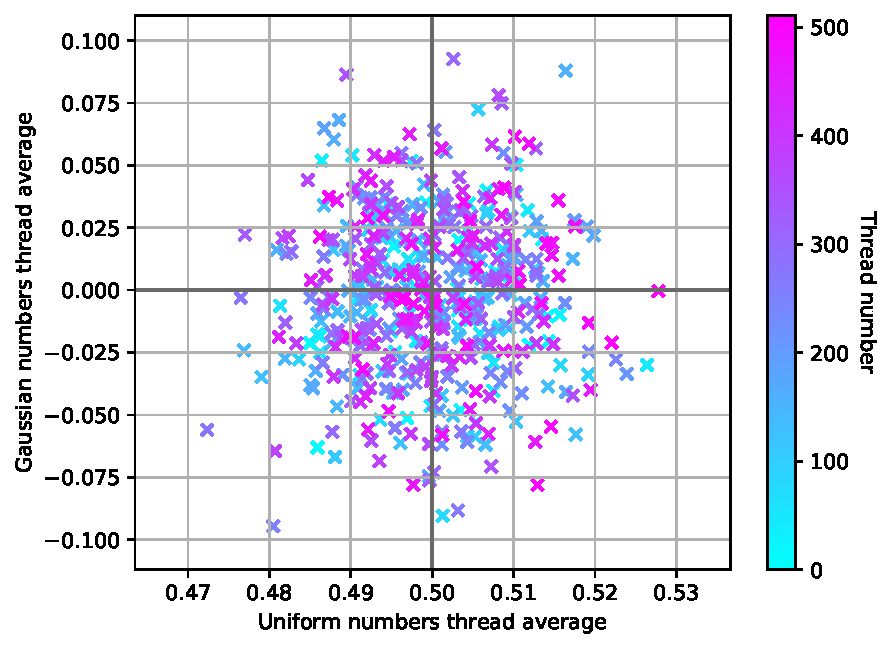
\includegraphics[scale=0.5]{graphs/CorrelationTests_UniAvgVsGaussAvg.pdf}
  \caption{}
  \label{fig:unigauss_avg}
\end{subfigure}%
\begin{subfigure}{.5\textwidth}
  \centering
  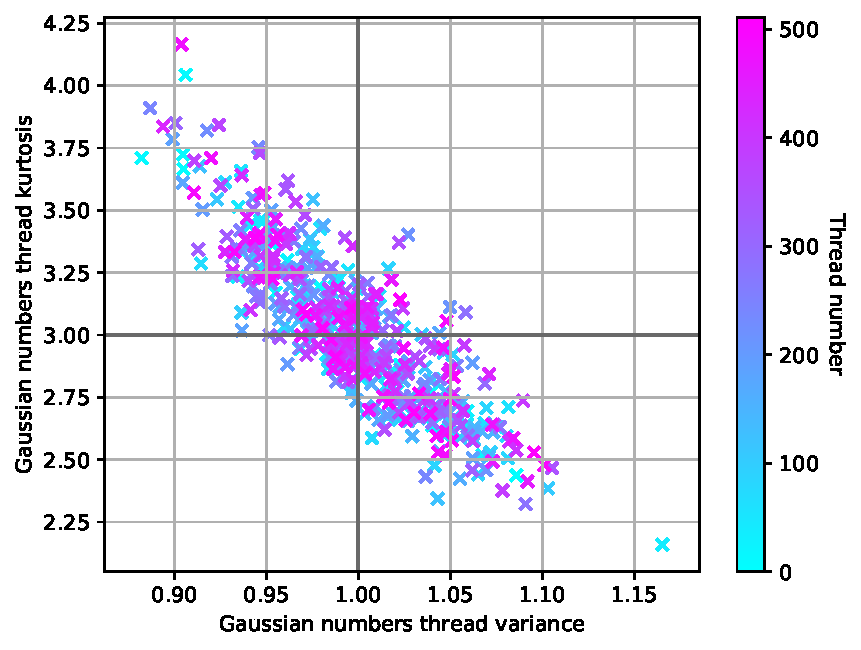
\includegraphics[scale=0.5]{graphs/CorrelationTests_KurtosisVsVariance.pdf}
  \caption{}
  \label{fig:variance_kurt}
\end{subfigure}
\caption{Dispersione di valori medi dei flussi di numeri pseudcasuali generati da ciascun \textit{thread} della GPU, il cui numero da 0 a 511 è indicato in scala cromatica da \textit{ciano} a \textit{magenta}. \textit{(a)} Dispersione delle medie dei numeri casuali generati nell'intervallo $[0,1]$ (ascissa) e dei numeri estratti da una distribuzione normale di media nulla e varianza unitaria (ordinata); \textit{(b)} dispersione di varianza e curtosi dei numeri estratti dalla medesima distribuzione normale di cui sopra. Le rette in \textit{grigio} evidenziano i valori teorici attesi per le quantità rappresentate: $\frac{1}{2}$ per la media di numeri uniformi, $0$, $1$ e $3$ per media, varianza e curtosi della distribuzione gaussiana.} 
\end{figure}

Per cominciare, in Figura \ref{fig:unigauss_avg} sono riportate le medie in ciascun \textit{thread} dei valori assunti dai numeri estratti uniformemente (in ascissa) e dai numeri estratti gaussianamente (in ordinata); come evidenziato dalla scala cromatica che indica il numero di \textit{thread}, la dispersione delle medie rispetto ai valori attesi indicati dalle rette in grigio non presenta asimmetrie significative. Un discorso analogo può essere fatto per la Figura \ref{fig:variance_kurt}, che riporta in ascissa la varianza
\begin{equation}
    \sigma^2 = \braket{{\left(r-\braket{r}\right)}^2}
    \label{eq:variance}
\end{equation}
e in ordinata la curtosi
\begin{equation}
    \text{Kurt}[r] = \frac{\braket{{\left(r-\braket{r}\right)}^4}}{\sigma^4}
    \label{eq:kurtosis}
\end{equation}
dei numeri generati gaussianamente, fatto salvo il \textit{caveat} che le due variabili sono evidentemente anticorrelate per la definizione di curtosi.

\begin{figure}[t]
\centering
\begin{subfigure}{.5\textwidth}
  \centering
  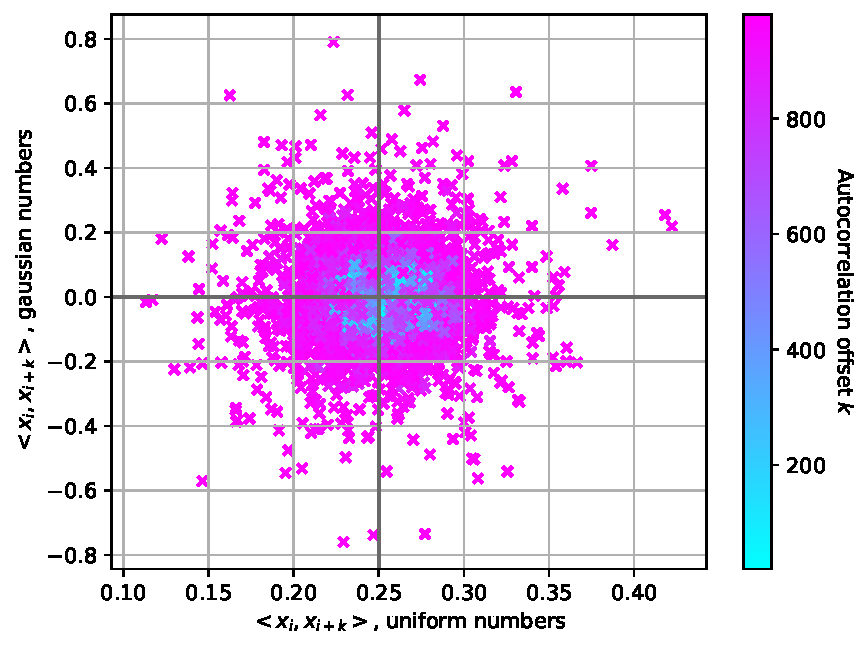
\includegraphics[scale=0.5]{graphs/CorrelationTests_IntraStreamCorrelations.pdf}
  \caption{}
  \label{fig:intra_corr}
\end{subfigure}%
\begin{subfigure}{.5\textwidth}
  \centering
  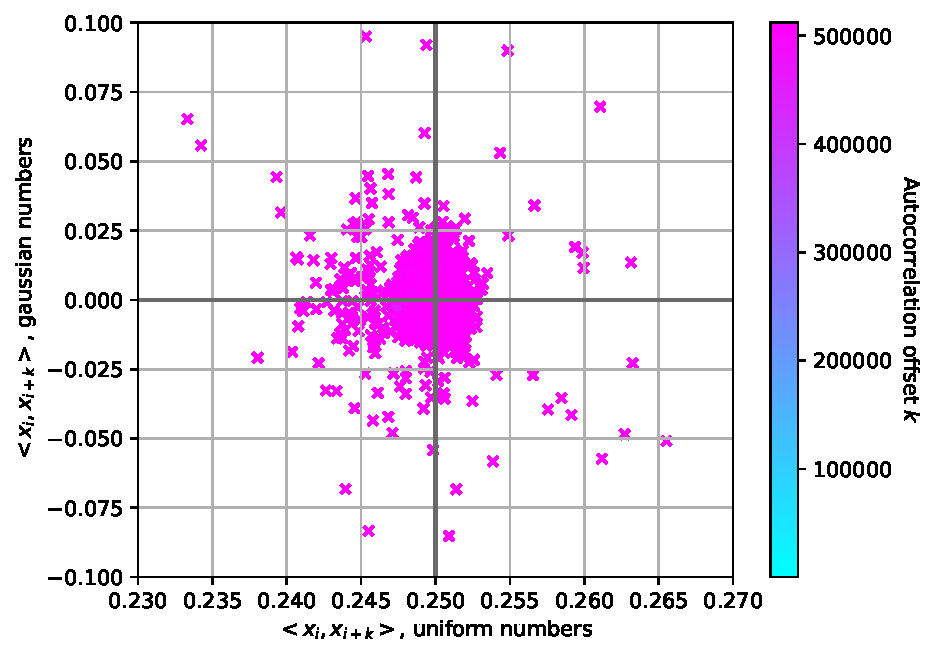
\includegraphics[scale=0.5]{graphs/CorrelationTests_InterStreamCorrelations.pdf}
  \caption{}
  \label{fig:inter_corr}
\end{subfigure}
\caption{Confronto tra autocorrelazioni $\braket{x_i x_{i+k}}$ nei casi di \textit{(a)} controllo \textit{intra-stream} sui flussi prodotti dai 512 \textit{thread}, e \textit{(b)} controllo \textit{inter-stream} effettuato su un singolo \textit{superstream} definito come in EQUAZIONE. In ascissa è riportata l'autocorrelazione nei flussi di numeri estratti uniformemente nell'intervallo $[0,1]$, in ordinata l'autocorrelazione dei numeri estratti secondo la distribuzione normale di media nulla e varianza unitaria; in scala cromatica da \textit{ciano} a \textit{magenta} è riportato il valore di $k$, mentre le rette in \textit{grigio} riportano i valori attesi ($\frac{1}{4}$ per la correlazione tra i numeri uniformi, $0$ per quella tra i numeri gaussiani).}
\end{figure}

Più spinoso è il caso della \textit{correlazione} $\braket{x_i x_{i+k}}$, dove $k$ è detto \textit{offset}. In Figura \ref{fig:intra_corr} è riportata la correlazione \textit{intra-stream} per i numeri distribuiti uniformemente (ascissa) e gaussianamente (ordinata). La scala cromatica questa volta indica l'\textit{offset} $k$, evidenziando come per $k$ elevati la dispersione dei risultati rispetto ai valori attesi (in grigio) sia fisiologicamente superiore in quanto sono disponibili meno numeri su cui effettuare la media. Ciononostante la distribuzione rimane visibilmente simmetrica e, pur non essendo evidenziati i risultati dei singoli \textit{thread}, studi in questa direzione non hanno evidenziato parzialità.

La Figura \ref{fig:inter_corr} riporta risultati secondo il medesimo schema della precedente applicati a un <<\textit{super-stream}>> ottenuto combinando tutti i 512 \textit{thread} secondo la formula
\begin{equation}
    w_{k=iN+j} = r_j^i,
    \label{eq:superstream}
\end{equation}
dove $j=1,...,512$ è l'indice di \textit{thread} e $i=1,...,1000$ è l'indice di numero generato. Se i numeri gaussiani preservano una distribuzione simmetrica intorno alla correlazione attesa, in quelli uniformi spicca una polarizzazione a favore di valori leggermente inferiori a $\frac{1}{4}$.

\begin{figure}[t]
\centering
\begin{subfigure}{.5\textwidth}
  \centering
  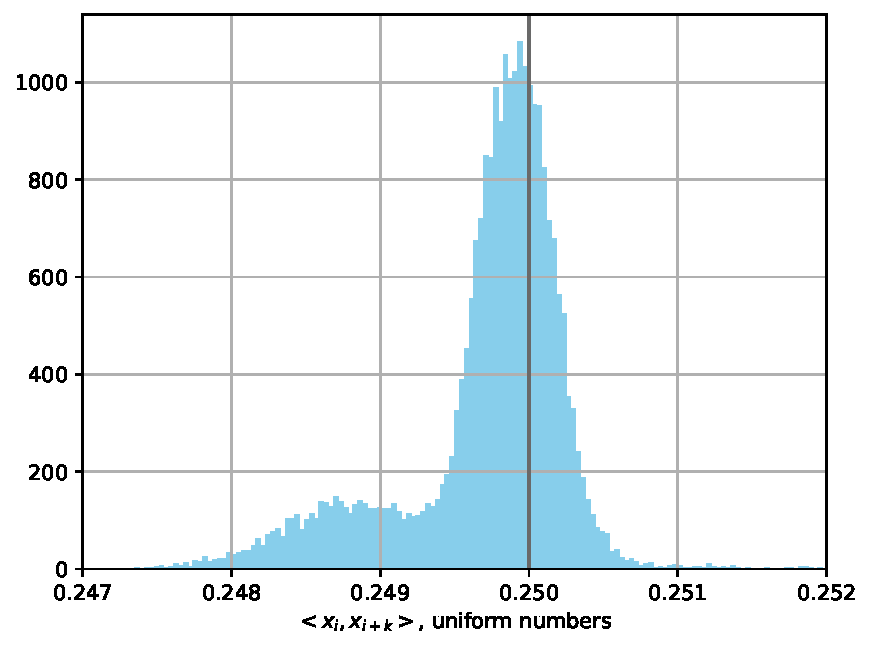
\includegraphics[scale=0.5]{graphs/CorrelationTests_UniformInterStreamAutocorrelationHistogram.pdf}
  \caption{}
  \label{fig:inter_uni_autocorr_histo}
\end{subfigure}%
\begin{subfigure}{.5\textwidth}
  \centering
  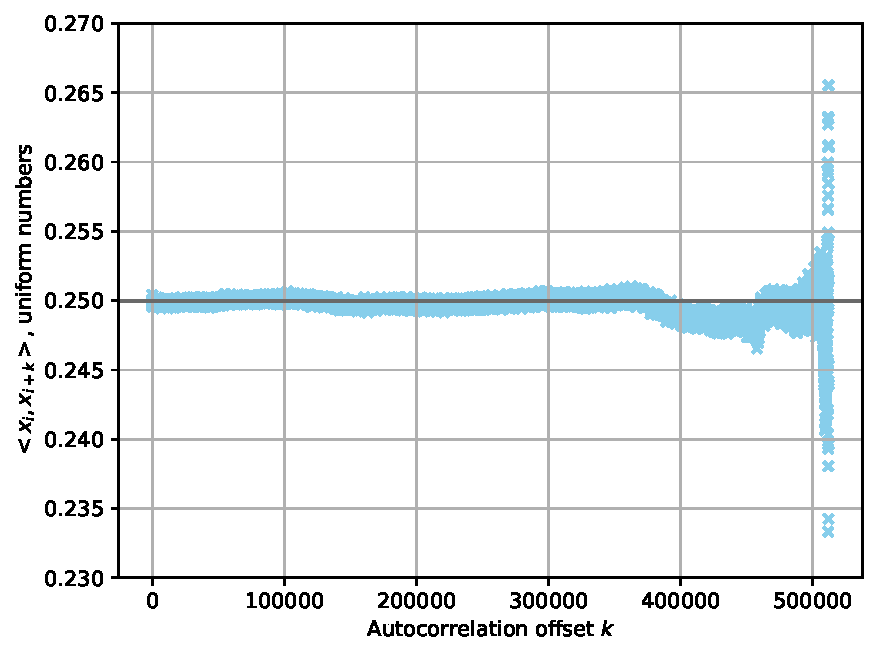
\includegraphics[scale=0.5]{graphs/CorrelationTests_UniformInterStreamAutocorrelationVsOffset.pdf}
  \caption{}
  \label{fig:inter_uni_autocorr_offset}
\end{subfigure}
\caption{\textit{(a)} Istogramma delle autocorrelazioni $\braket{x_i x_{i+k}}$ \textit{inter-stream} del flusso di numeri pseudocasuali estratti uniformemente nell'intervallo $[0,1]$; \textit{(b)} andamento delle correlazioni in funzione dell'\textit{offset} $k$.}
\end{figure}

Per indagare più a fondo questa distorsione abbiamo riportato in Figura \ref{fig:inter_uni_autocorr_histo} un istogramma delle correlazioni \textit{inter-stream} dei numeri uniformi e in Figura \ref{fig:inter_uni_autocorr_offset} il suo andamento in funzione di $k$. Da questi grafici è evidente come il picco secondario appaia per \textit{offset} particolarmente alti; ciononostante, anche l'andamento prima dell'anomalia presenta una forma vagamente oscillatoria, evidenziando come il flusso di numeri pseudocasuali non soddisfi pienamente la richiesta di autoindipendenza.

\begin{figure}[t]
\centering
\begin{subfigure}{.5\textwidth}
  \centering
  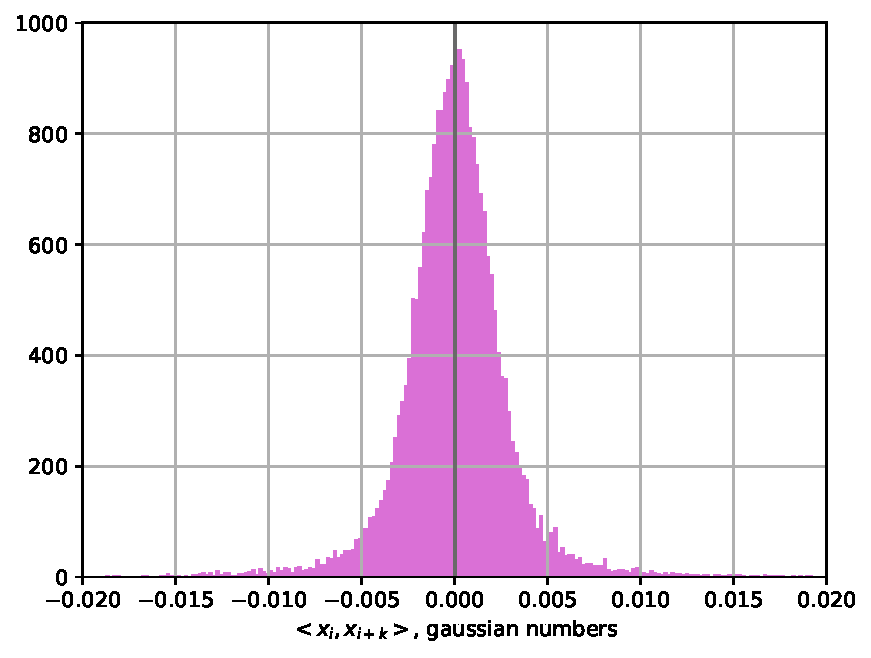
\includegraphics[scale=0.5]{graphs/CorrelationTests_GaussInterStreamAutocorrelationHistogram.pdf}
  \caption{}
  \label{fig:inter_gauss_autocorr_histo}
\end{subfigure}%
\begin{subfigure}{.5\textwidth}
  \centering
  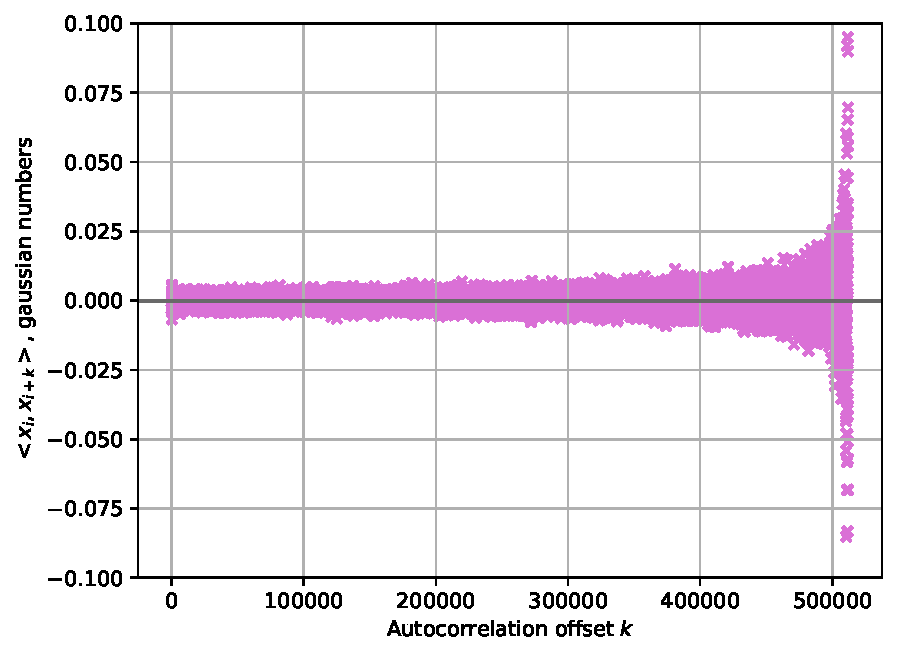
\includegraphics[scale=0.5]{graphs/CorrelationTests_GaussInterStreamAutocorrelationVsOffset.pdf}
  \caption{}
  \label{fig:inter_gauss_autocorr_offset}
\end{subfigure}
\caption{\textit{(a)} Istogramma delle autocorrelazioni $\braket{x_i x_{i+k}}$ \textit{inter-stream} del flusso di numeri pseudocasuali estratti uniformemente secondo una distribuzione normale di media nulla e varianza unitaria; \textit{(b)} andamento delle correlazioni in funzione dell'\textit{offset} $k$.}
\end{figure}

Ciononostante, le analoghe Figure \ref{fig:inter_gauss_autocorr_histo} e \ref{fig:inter_gauss_autocorr_offset} evidenziano come, pur essendo i numeri gaussiani generati a partire da quelli uniformi, in essi sia essenzialmente assente ogni spettro di autocorrelazione. Poiché le variabili gaussiane sono quelle di reale interesse, i controlli effettuati avvalorano l'indipendenza e l'affidabilità delle nostre simulazioni.

\section{(B-3) \textit{Pricing} dell'opzione \textit{performance corridor}} \label{sec:pc_pricing}
In questa sezione riportiamo gli studi sull'andamento del prezzo dell'opzione \textit{performance corridor} al variare di alcuni parametri chiave delle simulazioni.

\subsection{(B-3-a) Dipendenza del prezzo dalle date di rilevazione e dal numero di simulazioni}

\begin{figure}[t]
    \centering
    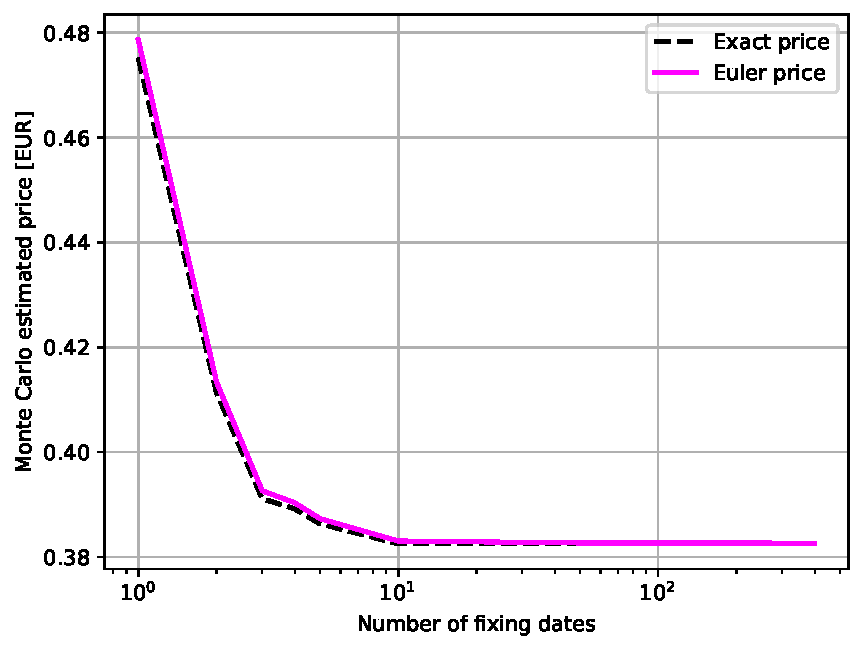
\includegraphics[scale=0.5]{graphs/OptionPriceVsM_PriceVsM_N100mln.pdf}
    \caption{Confronto dell'andamento del prezzo dell'opzione \textit{performance corridor} in funzione del numero di date di rilevazione calcolato secondo lo schema di Eulero (\textit{magenta}) e secondo lo schema esatto (\textit{nero}, \textit{tratteggiato}).}
    \label{fig:exactvseuler_M}
\end{figure}

In primo luogo abbiamo studiato la dipendenza del prezzo dell'opzione dal numero di date di rilevazione, verificando in particolare l'effetto che può indurre su eventuali discrepanze tra i risultati calcolati con lo schema esatto e lo schema di Eulero. In Figura \ref{fig:exactvseuler_M} è riportato il confronto tra due curve di prezzi in questione per $N={10}^8$ simulazioni; pur seguendo la medesima evoluzione e convergendo per campionamenti fitti, appare visibile una discrepanza non trascurabile quando la distanza temporale tra le date è maggiore.

\begin{figure}[t]
    \centering
    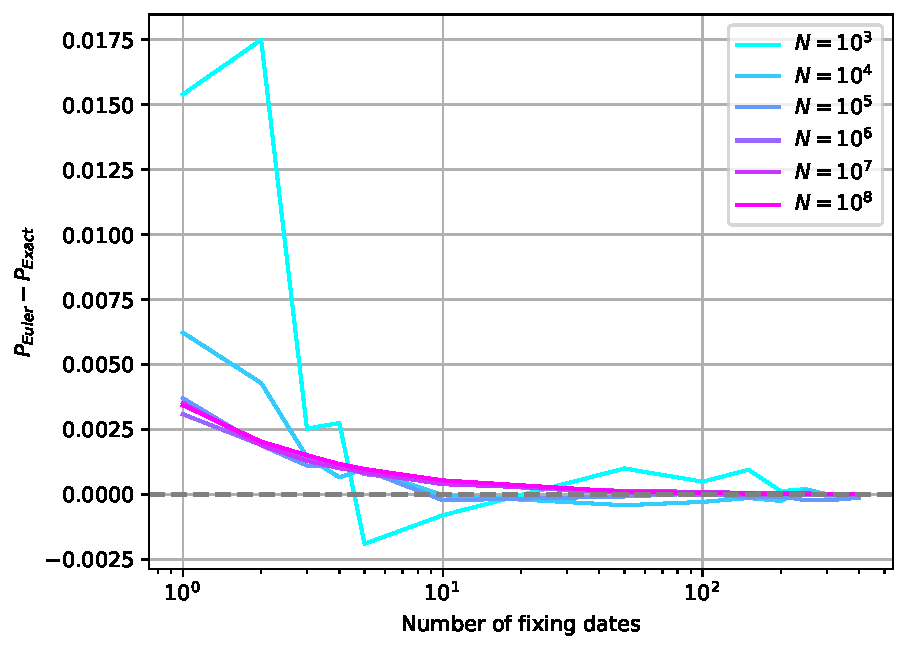
\includegraphics[scale=0.5]{graphs/OptionPriceVsM_DiscrepancyVsM_WithDifferentNs.pdf}
    \caption{Differenza tra i prezzi dell'opzione \textit{performance corridor} calcolati secondo lo schema di Eulero e secondo lo schema esatto in funzione del numero di date di rilevazione; da \textit{ciano} a \textit{magenta} curve con numero crescente di simulazioni da ${10}^3$ a ${10}^8$, in \textit{grigio tratteggiato} il valore asintotico di discrepanza nulla.}
    \label{fig:ex_eul_discrep_M}
\end{figure}

La natura di questa differenza tra i prezzi calcolati secondo le due formule emerge con più chiarezza in Figura \ref{fig:ex_eul_discrep_M}, dove è rappresentata in funzione delle densità di campionamento per diversi ordini di grandezza di simulazioni effettuate (in scala cromatica da ciano a magenta). Al crescere del numero di simulazioni, le discrepanze convergono stabilmente a una curva nonostante, come discusso più a fondo in Sezione \ref{sec:errorstudies}, l'errore Monte Carlo scali come $\epsilon_{MC}\propto N^{-\frac{1}{2}}$. Questa constatazione anticipa i limiti di applicabilità dello schema di Eulero per date di rilevazione troppo ridotte, che saranno approfonditi in Sezione \ref{sec:limits}.

\subsection{(B-3-b) Dipendenza del prezzo dal valore di $B$}

\begin{figure}[t]
    \centering
    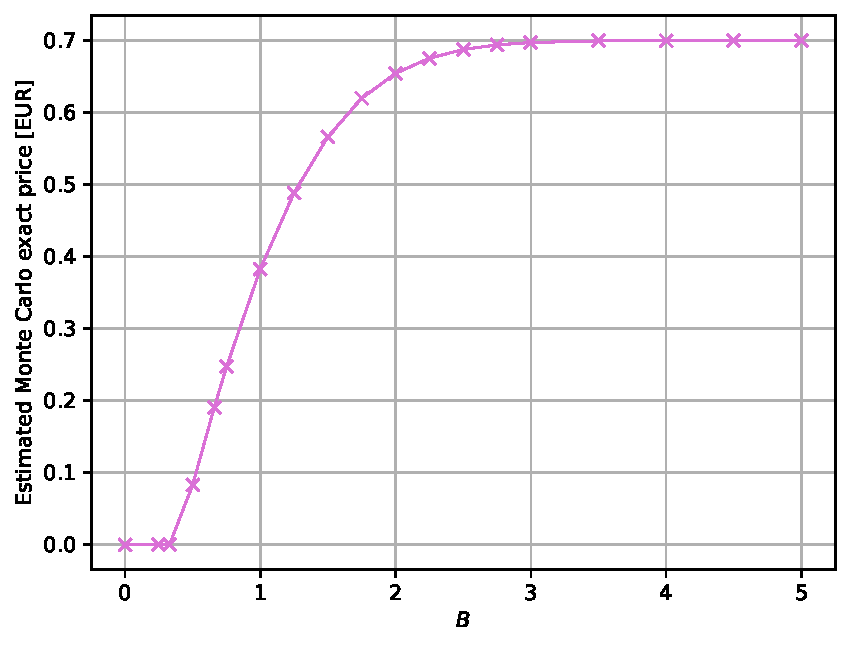
\includegraphics[scale=0.5]{graphs/OptionPriceVsB_PriceVsB_N200mln.pdf}
    \caption{Andamento del prezzo dell'opzione \textit{performance corridor} stimato secondo lo schema esatto in funzione del parametro $B$ che determina l'altezza della barriera.}
    \label{fig:price_vs_b}
\end{figure}

In Figura \eqref{fig:price_vs_b} è rappresentato l'andamento del prezzo stimato dell'opzione secondo lo schema esatto al variare del parametro $B$ per rilevazione giornaliera ($m=365$) del rendimento logaritmico. Un'interpretazione euristica del grafico è immediata osservando che il termine $\frac{1}{m} \sum_i P_i$ nella \ref{eq:performancecorridor_payoff} corrisponde alla percentuale di date in cui il modulo del rendimento del sottostante è rimasto confinato all'interno della barriera: per $B -> 0$ il <<corridoio>> è infinitesimo e il \textit{payoff} risulta nullo; esso cresce poi all'aumentare dell'altezza della barriera fino a raggiungere un valore di saturazione $\approx 1-K$ ($K=0.3$ nelle simulazioni in figura), ovvero quando il rendimento non eccede mai il valore fissato. Una deduzione più rigorosa di questi limiti asintotici sarà fornita nel Capitolo \ref{cap:exactformulas}.


\section{(B-4) Studi sull'errore Monte Carlo} \label{sec:errorstudies}
Se nella precedente sezione ci siamo concentrati sulle variazioni in prezzo simulato, qui affronteremo invece l'impatto dei medesimi parametri sull'entità dell'errore della stima Monte Carlo come definito nella \eqref{eq:mcerror}.

\subsection{(B-4-a) Dipendenza dell'errore dalle date di rilevazione e dal numero di simulazioni} \label{sec:error_vs_m_and_N}

\begin{figure}[t]
\centering
\begin{subfigure}{.5\textwidth}
  \centering
  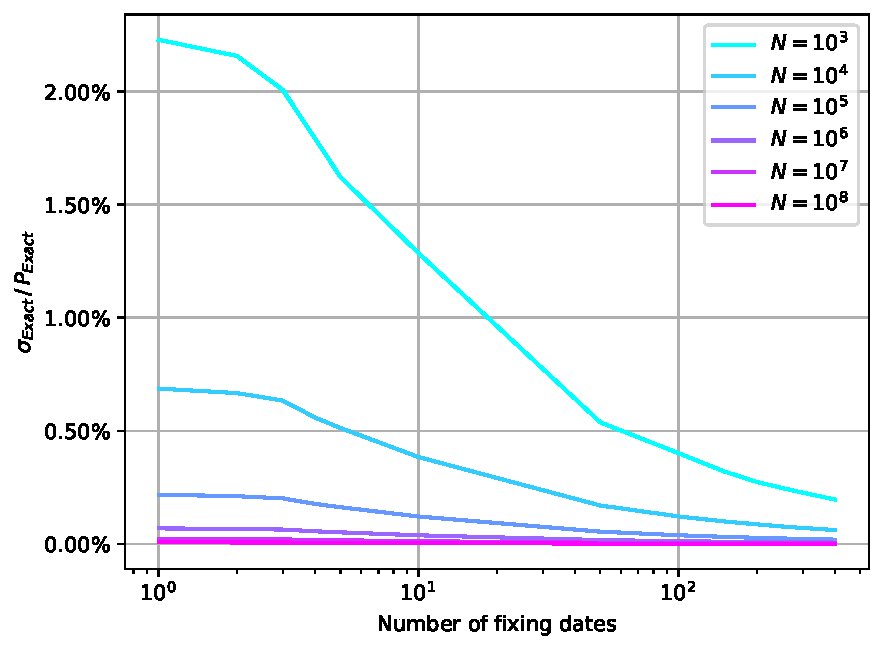
\includegraphics[scale=0.5]{graphs/OptionPriceVsM_ExactErrorVsM_WithDifferentNs.pdf}
  \caption{}
  \label{fig:exact_error_M}
\end{subfigure}%
\begin{subfigure}{.5\textwidth}
  \centering
  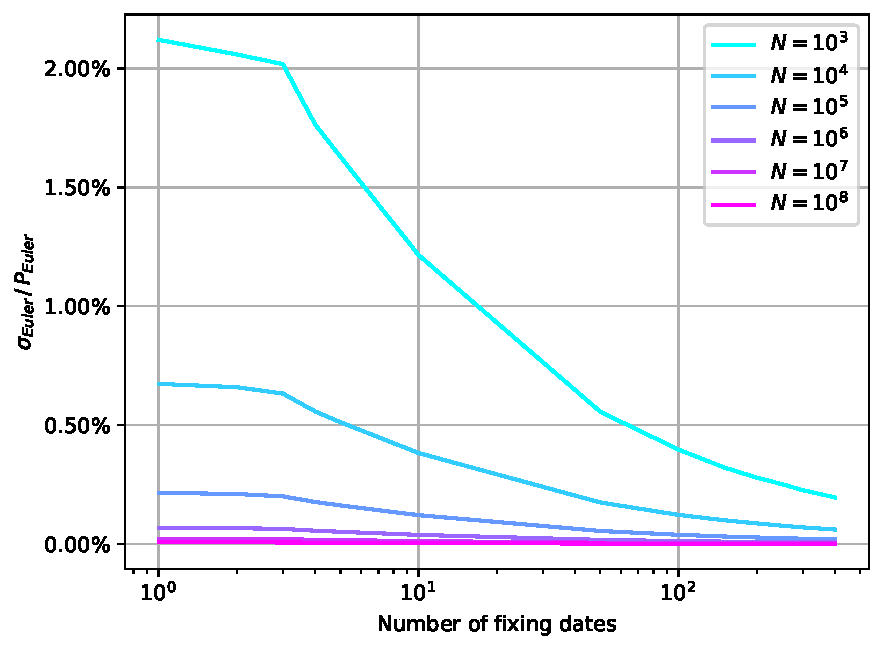
\includegraphics[scale=0.5]{graphs/OptionPriceVsM_EulerErrorVsM_WithDifferentNs.pdf}
  \caption{}
  \label{fig:euler_error_M}
\end{subfigure}
\caption{Andamento dell'errore relativo Monte Carlo in funzione del numero di date di rilevazione rispetto al prezzo calcolato \textit{(a)} secondo lo schema esatto e \textit{(b)} secondo lo schema di Eulero; curve di colore da \textit{ciano} a \textit{magenta} corrispondono a un numero crescente di simulazioni da ${10}^3$ a ${10}^8$.}
\end{figure}

Le Figure \ref{fig:exact_error_M} e \ref{fig:euler_error_M} riportano l'andamento dell'errore relativo in percentuale del prezzo stimato rispettivamente secondo lo schema esatto e lo schema di Eulero in funzione del numero di date rilevazione per numero crescente di simulazioni. In esse è evidenziata una doppia dipendenza: l'errore tende a diminuire sia per un numero di simulazioni maggiore che per un campionamento di rilevazione più fitto. Se la prima è una caratteristica comune a tutte le simulazioni Monte Carlo in generale, il cui errore scala come $\frac{1}{\sqrt{N}}$, il secondo è un comportamento peculiare dell'opzione \textit{performance corridor} che non si riscontra in controlli analoghi effettuati su opzioni \textit{plain vanilla}.

Una spiegazione della dipendenza da $m$ si trova interpretando il calcolo del \textit{payoff} come da equazioni \eqref{eq:performancecorridor_payoff} e \eqref{eq:performancecorridor_barrier} nell'ottica di un processo di Bernoulli, ossia un processo costituito da una serie di eventi indipendenti detti \textit{prove di Bernoulli} che hanno come soli possibili risultati un successo (probabilità $p$) o un fallimento (probabilità $1-p$). Nel caso dell'opzione \textit{performance corridor}, le prove in questione sono le <<estrazioni>> del valore di $P_i$ nelle $m$ date di rilevazione, le quali hanno probabilità di successo ($P_i=1$) pari a
\begin{equation}
\begin{aligned}
    p &= P(P_i = 1) = P\left(\left| \frac{1}{\sqrt{\Delta t}} \ln{\frac{S_{i+1}}{S_i}} \right| < B \sigma\right) \\
    &= P\left(\left| \left(r - \frac{\sigma^2}{2}\right)\sqrt{\Delta t} + \sigma w \right| < B \sigma\right).
    \label{eq:success_prob_bernoulli}
\end{aligned}
\end{equation}

Poiché $w$ è una variabile estratta da una distribuzione normale di media nulla e varianza unitaria, possiamo usare la corrispondente funzione di distribuzione cumulativa per definire la probabilità $P(w \leq X)$\footnote{La probabilità calcolata tramite funzione cumulativa è per $w$ minore \textit{o uguale} a un certo valore, mentre la probabilità che cerchiamo nella \eqref{eq:success_prob_bernoulli} è esclusivamente minore. Ciò non è un problema, poiché la probabilità puntuale in una funzione di densità di probabilità è nulla.}
\begin{equation}
    P(w \leq x) = \mathcal{N}[x] = \frac{1}{\sqrt{2\pi}} \int_{-\infty}^x{e^{-\frac{1}{2} t^2} dt}
    \label{eq:cumulative_gaussian}
\end{equation}
e riscrivere la probabilità \eqref{eq:success_prob_bernoulli} come
\begin{equation}
    p = \mathcal{N}\left[B - \left(r - \frac{\sigma^2}{2}\right)\frac{\sqrt{\Delta t}}{\sigma} \right] \cdot \left(1 - \mathcal{N}\left[- B - \left(r - \frac{\sigma^2}{2}\right)\frac{\sqrt{\Delta t}}{\sigma} \right]\right).
    \label{eq:success_prob_cumul}
\end{equation}

La probabilità di avere $n$ successi in $m$ date di rilevazione è data dalla distribuzione binomiale, la cui varianza è
\begin{equation}
    \text{Var}[n] = mp(1-p).
    \label{eq:binomial_variance}
\end{equation}

Assumendo che la scelta di $B$ e $K$ sia tale da non rendere mai negativo il termine $\frac{1}{m} \sum_{i=0}^{m-1}{P_i} - K$ nella \eqref{eq:performancecorridor_payoff}, si può trascurare la presenza della parte positiva nel calcolo dell'errore previsto; per $N$ simulazioni abbiamo dunque
\begin{equation}
    \epsilon^2_{\text{teor}} = \frac{1}{N} \text{Var}\left[\frac{n}{m} - K\right] = \frac{1}{Nm} p(1-p).
    \label{eq:error_theoretical_squared}
\end{equation}

\begin{figure}[t]
    \centering
    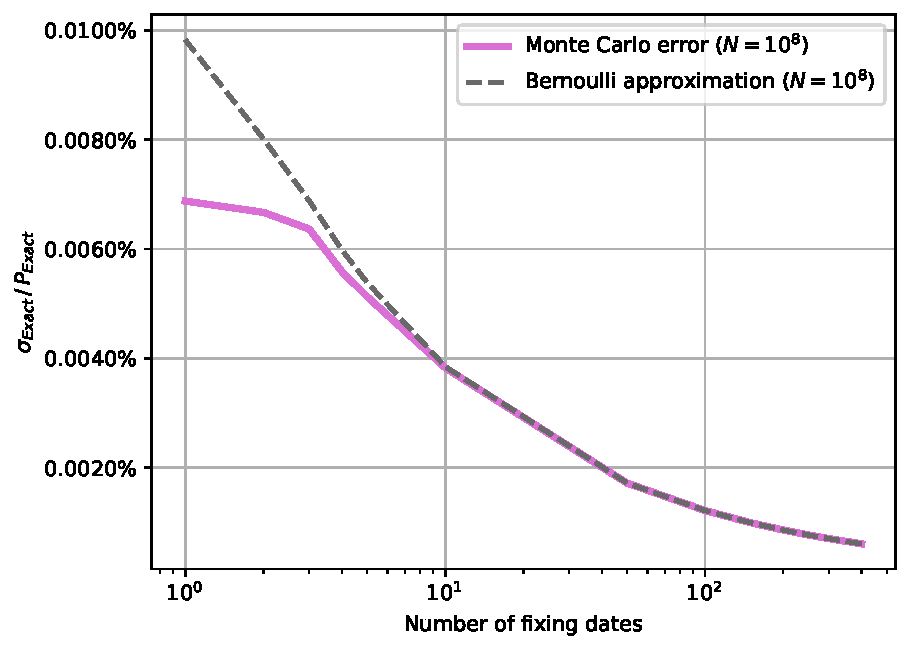
\includegraphics[scale=0.5]{graphs/OptionPriceVsM_ExactErrorVsM_N108.pdf}
    \caption{Andamento dell'errore relativo Monte Carlo (in \textit{magenta}) in funzione del numero di date di rivelazione rispetto al prezzo calcolato secondo lo schema esatto, per $N={10}^8$ simulazioni dell'evoluzione del sottostante; in \textit{grigio tratteggiato} le previsioni teoriche ottenute modellizzando il superamento della barriera con un processo di Bernoulli.}
    \label{fig:theoretical_vs_experimental_error}
\end{figure}

A titolo di esempio, in Figura \ref{fig:theoretical_vs_experimental_error} è riportato il confronto tra modello teorico ed errore sperimentale per $N={10}^8$ simulazioni, con una confluenza efficace già per $m \gtrsim 5$.

\subsection{(B-4-b) Dipendenza dell'errore dal valore di $B$}

\begin{figure}[t]
    \centering
    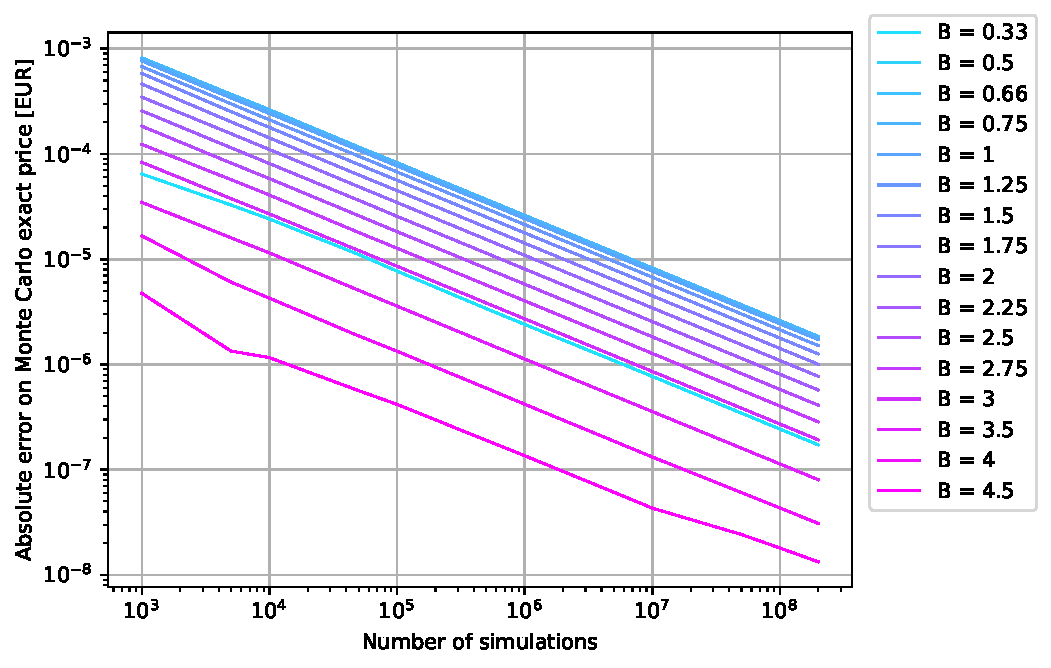
\includegraphics[scale=0.5]{graphs/OptionPriceVsB_ExactErrorVsN_WithAllBs.pdf}
    \caption{Errore assoluto Monte Carlo rispetto al prezzo calcolato secondo lo schema esatto in funzione del numero di simulazioni effettuate; curve di colore da \textit{ciano} a \textit{magenta} corrispondono a valori crescenti del parametro $B$.}
    \label{fig:error_vs_B}
\end{figure}

Come mostrato in Figura \ref{fig:error_vs_B} nel caso dello schema esatto, l'errore assoluto sulla stima prezzo Monte Carlo presenta anche una dipendenza dal valore di $B$, ovvero dall'altezza della barriera. La scala bilogaritmica evidenzia infatti una legge di scala dell'errore del tipo
\begin{equation}
    \epsilon_\text{MC} = \frac{H(B)}{\sqrt{N}},
    \label{eq:h_of_b}
\end{equation}
dove $N$ è il numero di simulazioni e $H$ una costante moltiplicativa che dipende da fattori quali i dati di mercato, le condizioni contrattuali e da eventuali tecniche di riduzione della varianza.

\begin{figure}[t]
    \centering
    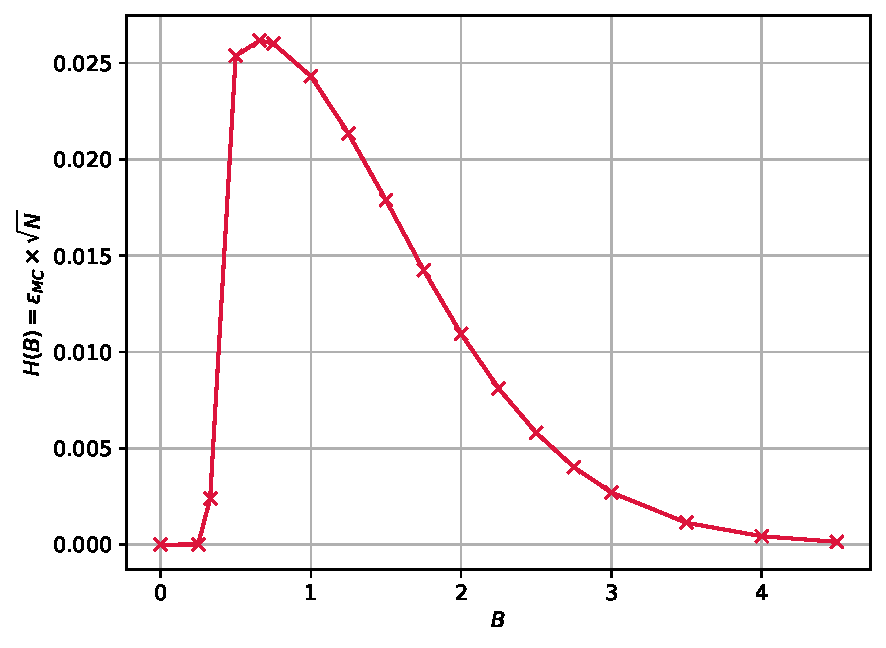
\includegraphics[scale=0.5]{graphs/OptionPriceVsB_HBVsB.pdf}
    \caption{Andamento del valore della costante moltiplicativa $H(B)$ nell'equazione \eqref{eq:h_of_b} in funzione di $B$.}
    \label{fig:HB_vs_B}
\end{figure}

Abbiamo estrapolato la dipendenza di $H$ dal valore di $B$ invertendo la \eqref{eq:h_of_b} e mediando in $N$; la curva risultante è mostrata in Figura \ref{fig:HB_vs_B}. L'andamento individuato trova una sua interpretazione osservando che la formula per il calcolo dell'errore Monte Carlo \eqref{eq:mcerror} lo lega, tra le altre cose, alla dispersione dei prezzi stimati. È sufficiente confrontare la curva in questione con quella del prezzo al variare di $B$ riportata in Figura \ref{fig:price_vs_b} per intuire che, per valori molto ridotti o elevati di $B$, il confinamento del rendimento logaritmico del sottostante è rispettivamente nullo o totale e in ambo i casi la dispersione dei \textit{payoff} calcolati secondo la \eqref{eq:performancecorridor_payoff} tende asintoticamente a zero. Quando l'ampiezza del corridoio cresce abbastanza da permettere ai \textit{payoff} di iniziare a variare, l'errore Monte Carlo sale molto rapidamente raggiungendo un picco per $B\approx 1.25$; a quel punto aumentare ulteriormente la barriera riduce la probabilità che $\frac{1}{\sqrt{\Delta t}}\ln{\frac{S_{i+1}}{S_i}}$ la ecceda, il \textit{payoff} tende alla saturazione e la variabilità in calo induce una diminuzione di $\epsilon_\text{MC}$ che tende nuovamente a zero.

\section{(B-5) Studi sui tempi di esecuzione} \label{sec:comptime}
\subsection{(B-5-a) Analisi dei tempi di esecuzione in GPU}
Come anticipato nella Sezione \ref{sec:hardware} relativa alle specifiche hardware, i dati per lo studio dei tempi di esecuzione sono stati raccolti tramite la scheda grafica di modello \verb|Tesla C2075|.

La scelta è stata dettata dalla volontà di visualizzare le attese discontinuità <<a gradini>> nell'andamento dei tempi di esecuzione in funzione del numero di blocchi istanziati. Ogni scheda grafica ha infatti un certo numero di multiprocessori che limitano la quantità di blocchi da poter chiamare contemporaneamente. Nel momento in cui si eccede questa quantità, la GPU deve rinunciare a eseguire in parallelo tutti i processi e l'esecuzione viene scorporata in più fasi successive fino al raggiungimento del numero di blocchi richiesto.
Il modello \verb|Tesla P100-PCIE-12GB| è risultato eccessivamente performante rispetto alla CPU montata sullo stesso nodo: garantendo la possibilità di gestire in contemporanea fino a 56 blocchi, tale scheda richiederebbe di istanziarne un numero piuttosto elevato per poter osservare l'andamento a gradini. L'esecuzione su CPU relativa a una simile simulazione avrebbe così tempistiche proibitive.

In Figura \ref{fig:gpucomptime} viene rappresentato il tempo di esecuzione GPU relativo a simulazioni con numero diverso di date di rilevazione. A ogni \textit{thread} sono demandate 1000 simulazioni, così da rendere il calcolo sufficientemente intensivo.

\begin{figure}[t]
    \centering
    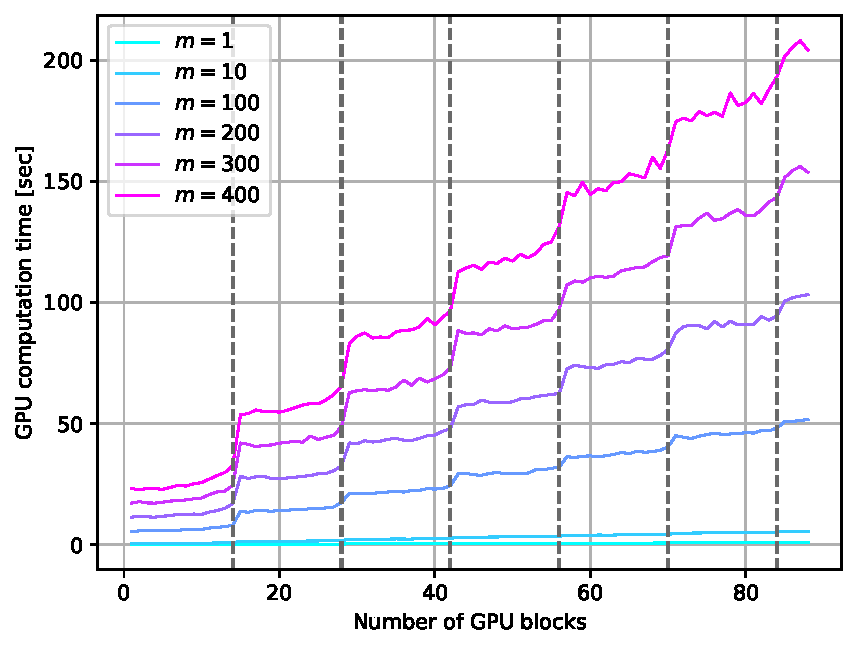
\includegraphics[scale=0.5]{graphs/ComputationTime_Tesla_GPUTimeVsNOfBlocks_VariousM_1000SimsPerThread.pdf}
    \caption{Tempi di esecuzione dell'algoritmo su GPU al crescere del numero di blocchi per diverse densità di date di rilevazione. Nelle simulazioni cronometrate in ogni blocco erano istanziati 512 \textit{thread}, ciascuno incaricato di eseguire 1000 simulazioni dell'evoluzione del prezzo del sottostante.}
    \label{fig:gpucomptime}
\end{figure}


Le simulazioni per $m=1$ e $m=10$ hanno una velocità di esecuzione troppo alta per apprezzare la differenza al crescere del numero di blocchi. A partire da $m=20$ la tendenza crescente dei tempi e lo sviluppo non lineare diventano evidenti. Nel grafico abbiamo sottolineato la lunghezza dei singoli passi attraverso linee verticali tratteggiate a intervalli di 14 blocchi, cioè il numero massimo di blocchi coordinabili dalla nostra GPU. Per densità di date di rilevazione più alte si accentuano ulteriormente le discontinuità e l'altezza dei gradini, ma subentra un altro disturbo.

A partire da un dato scalino, il cui indice tende a decrescere per m crescente, la porzione di grafico tra un salto e l'altro risulta più irregolare e con una pendenza via via maggiore all'aumentare del numero di blocchi. Ciò comporta, in particolar modo nelle simulazioni con $m=300$ e $m=400$, una progressiva perdita della struttura a gradino. Questa sorta di interferenza potrebbe essere causata dal maggior numero di accessi in memoria. Per verificare questa ipotesi, abbiamo provato a ripetere il processo aumentando il numero di simulazioni per \textit{thread}, ottenendo risultati analoghi a quelli appena considerati. La nostra teoria sembra quindi ragionevole.

\subsection{(B-5-b) Analisi del fattore di guadagno GPU-CPU}

Nella Sezione introduttiva \ref{sec:code_generics} abbiamo visto come l'esecuzione di algoritmi parallelizzabili in GPU permetta di abbattere i tempi di calcolo sfruttando l'architettura a multiprocessori di tale apparecchiatura (si veda il Capitolo \ref{cap:cudacpp} per ulteriori approfondimenti). Dopo aver osservato come variano i tempi di esecuzione su GPU in funzione del numero di blocchi, ci occupiamo ora di effettuare un confronto tra le \textit{performance} di GPU e CPU per testare la convenienza del primo approccio rispetto al secondo.

Abbiamo a tal fine inserito in un grafico, Figura \ref{fig:gainfactor}, la dipendenza del fattore di guadagno, dato dal rapporto tra i tempi di esecuzione in CPU e i rispettivi tempi di esecuzione in GPU, dal numero di blocchi della simulazione considerata. In entrambi i casi i tempi sono stati calcolati per mezzo dell'<<orologio interno>> della GPU. 

\begin{figure}[t]
    \centering
    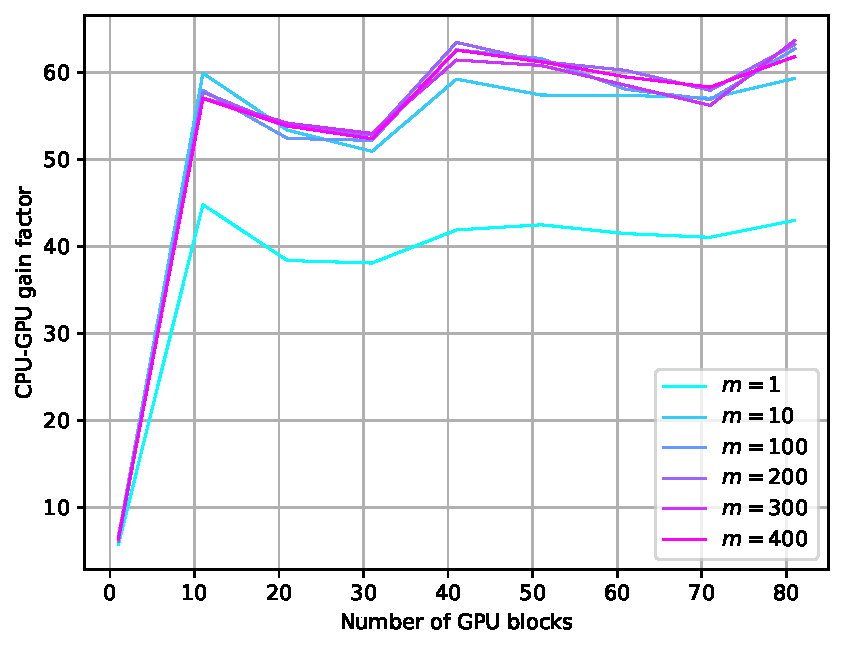
\includegraphics[scale=0.5]{graphs/GainFactor_Tesla_GainFactorVsBlocks_VariousM.pdf}
    \caption{Fattore di guadagno dell'algoritmo su GPU rispetto a quello su CPU al crescere del numero di blocchi per diverse densità di date di rilevazione; numero di \textit{thread} per blocco e simulazioni per \textit{thread} sono i medesimi che nella Figura \ref{fig:gpucomptime}}
    \label{fig:gainfactor}
\end{figure}

L'operazione è stata ripetuta per diversi valori di densità di date di rilevazione, individuate nel grafico da colori distinti nella gamma ciano-magenta. Il numero di \textit{thread} per blocco istanziati è di 512, a ogni \textit{thread} sono affidate 1000 simulazioni. 

La maggiore efficienza della GPU, coerentemente con le aspettative, risulta evidente per ogni valore di $m$. Tutti gli andamenti presentano un'iniziale fase di crescita, per poi stabilizzarsi attorno a un valore di $t_{CPU}/t_{GPU}$ diverso in base al numero di date di rilevazione considerato. Per $m=1$ il fattore di guadagno è di circa $40$. Gli altri sviluppi risultano piuttosto sovrapponibili, con un fattore di guadagno attorno a $60$ a tendenza leggermente crescente.

\section{(B-6) Limiti di applicabilità dello schema di Eulero} \label{sec:limits}

Gli studi sul prezzo dell'opzione \textit{performance corridor} condotti in Sezione \ref{sec:pc_pricing}, e in particolare il grafico in Figura \ref{fig:ex_eul_discrep_M}, hanno evidenziato come il metodo approssimato di Eulero \eqref{eq:eulerprice} non riesca a riprodurre in modo proficuo la formula esatta \eqref{eq:exactprice} per date combinazioni di numero di simulazioni $N$ e numero di date di rilevazione $m$.

Un fattore che contribuisce a questa distorsione sistematica è il fatto che, calcolando il prezzo secondo lo schema di Eulero, si incorre in una probabilità non nulla che il prezzo del sottostante diventi negativo. Data infatti la formula
\begin{equation}
    S(t_{i+1}) = S(t_i) \left(1 + r \Delta t + \sigma \sqrt{\Delta t} w\right),
    \label{eulerprice_repeat}
\end{equation}
il termine in parentesi sarà negativo qualora la variabile $w$ sia estratta con un valore
\begin{equation}
    w < w_{lim} \equiv - \frac{1+r \Delta t}{\sigma \sqrt{\Delta t}}.
\end{equation}
Come discusso in Sezione \ref{sec:error_vs_m_and_N}, la probabilità che ciò avvenga per una variabile estratta secondo una distribuzione normale di media nulla e varianza unitaria è
\begin{equation}
    P\left(S(t_{i+1})<0\right) = \mathcal{N}\left[w_{lim} \right],
    \label{eq:probability_negativeprice}
\end{equation}
dove $\mathcal{N}[x]$ è la funzione di distribuzione normale cumulativa definita come da \eqref{eq:cumulative_gaussian}. Posto $\Delta t = \frac{T}{m}$, si verifica facilmente che $w_{lim} \rightarrow 0$ per $m \rightarrow 0$ e $w_{lim} \rightarrow -\infty$ per $m \rightarrow +\infty$. Questo implica che è più probabile ottenere prezzi negativi per campionamenti più rarefatti, spiegando almeno in parte le discrepanze osservate tra schema di Eulero e schema esatto in tali situazioni.

\begin{figure}[t] 
    \centering
    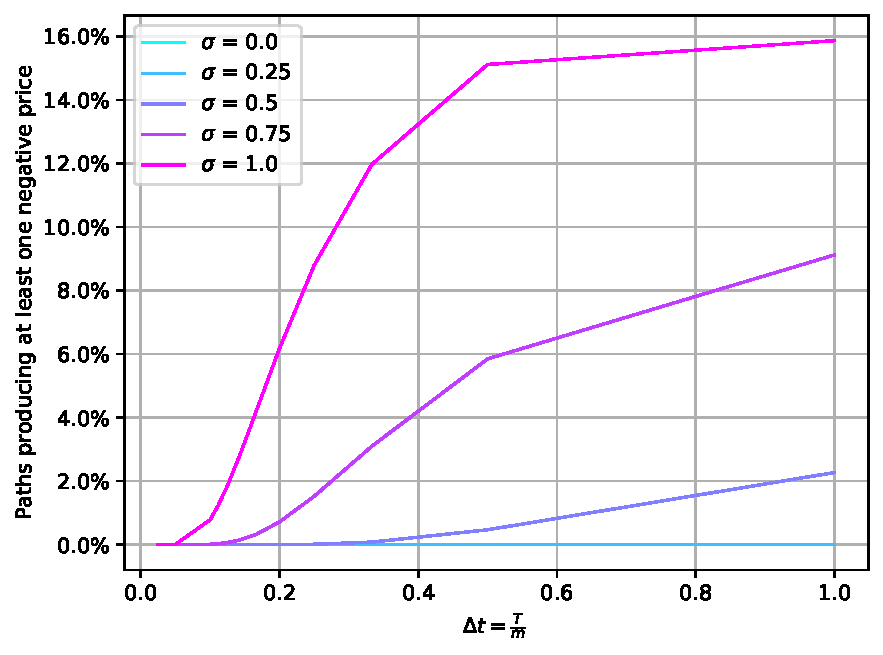
\includegraphics[scale=0.5]{graphs/NegativePrices_PercentageVsM_VariousSigmas.pdf}
    \caption{Percentuale di evoluzioni simulate del prezzo del sottostante che riportano almeno un'istanza di prezzo $S(t_i)$ negativo al variare della distanza temporale $\Delta t$ tra le date di rilevazione; curve di colore da \textit{ciano} a \textit{magenta} corrispondono a valori crescenti della volatilità $\sigma$ del mercato.}
    \label{fig:negativeprices}
\end{figure}

Altro fattore contributivo, come evidenziato dal grafico in Figura \ref{fig:negativeprices}, è dato dalla volatilità $\sigma$: si osserva infatti che accrescere il valore di quest'ultima incrementa anche la probabilità che nel corso della simulazione il prezzo sottostante diventi negativo almeno una volta, arrivando al $16\%$ per $\sigma=100\%$. Notiamo comunque che per $\sigma=25\%$, ovvero il nostro valore <<standard>>, l'incidenza di questa anomalia è estremamente bassa, e in generale per volatilità non patologiche già a $\Delta t \approx 0.2$ ($m=5$ se $T=1 \, \text{yr}$) questa incertezza sistematica nello schema di Eulero diventa trascurabile.

Tenendo in debita considerazione i risultati ottenuti negli studi in Sezione \ref{sec:pc_pricing}, possiamo concludere che lo schema di Eulero può essere un'approssimazione ottimale dello schema esatto, specie a livello di economia computazionale in quanto non necessita del calcolo di un'esponenziale, a patto di tenere sotto controllo le date di rilevazione e di avere a disposizione sufficiente statistica in modo da minimizzare la variabilità dei risultati. Evidenziamo in ogni caso che, per $N\approx 10^6$ simulazioni e $m = 100$ date di rilevazione (parametri più lassi di quelli da noi generalmente usati), la Figura \ref{fig:ex_eul_discrep_M} conferma che la convergenza tra le due formule è più che adatta ai nostri scopi, con compatibilità dei prezzi stimati entro $2\sigma_e \equiv 2\sqrt{\epsilon_\text{exact}^2 + \epsilon_\text{euler}^2}$.